\documentclass[12pt,a4paper]{article}
\usepackage[utf8]{inputenc}
\usepackage[spanish]{babel}
\usepackage{amsmath}
\usepackage{amsfonts}
\usepackage{amssymb}
\usepackage{makeidx}
\usepackage{graphicx}
\usepackage{lmodern}
\usepackage{fourier}
\usepackage[left=2cm,right=2cm,top=2cm,bottom=2cm]{geometry}
\author{Flores Macias Cesar Fabian}
\title{Segundo_Avance}
\begin{document}
\begin{center}

\includegraphics[width=16cm]{Imagenes/logo.png}  \\
\end{center}
\textbf{UNIVERSIDAD POLITECNICA DE LA ZONA METROPOLITANA DE GUADALAJARA}\\
\textit{CONEMATICA DE ROBOTS}\\
\textit{Maestro: Carlos Enrique Moran Garabito}\\
\textit{Alumnos: Flores Macias Cesar Fabian\\
Martinez Hernandez Samuel Caleb\\
Canales Ochoa Fabian\\
Gutierrez Chavez Amaury Efrain}\\
\begin{center}
BRAZO SCARA
\end{center}
Introducción\\
Un SCARA es un robot de cuatro grados de libertad con posicionamiento horizontal. Los Robots SCARA se conocen por sus rápidos ciclos de trabajo, excelente repetitividad, gran capacidad de carga y su amplio campo de aplicación.\\
\begin{center}
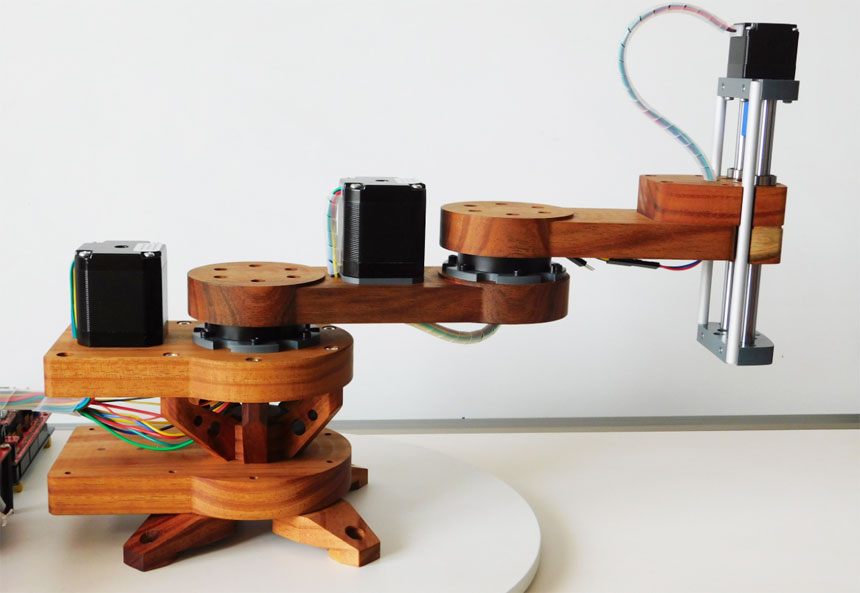
\includegraphics[width=7cm]{Imagenes/SC.jpg}\\1.0 Robot SCARA
\end{center}
El brazo SCARA presentado en el anterior reporte tiene fallas con respecto a diseño, funcionalidad, entre ellos se destacan: \\
\textbf{Diseño:}\\
Con respecto a la anterior base que solía ser alta semi circular, se ha decidido crear un nuevo diseño de forma mas sencilla y minimalista sin perder sustentabilidad, equilibro. El nuevo diseño de esta esta conformada por un tubo de aproximadamente de 2cm de diámetro y su interior hueco para poder realizar el cableado y conexión de los servomotores que darán movilidad al brazo.\\
\textbf{Servomotores:}\\
El motor que realizara el movimiento principal de 180o sera de forma cilindrica con un diametro de 1.87cm y el espacio restante con respecto al tuvo sera rellenado por un silicion a algun tipo de adesivo que resista las vivraciones de los mivimientos.\\
\begin{center}
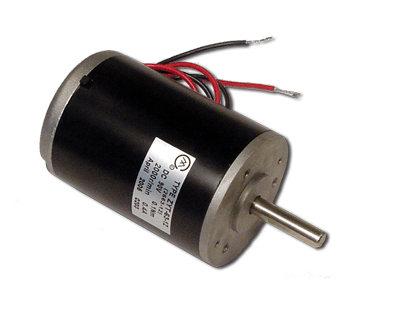
\includegraphics[scale=0.5]{Imagenes/M.png}\\1.1 Servomotor
\end{center}
Brazos con grados de libertad:\\
Los brazos con grados de libertad serán principalmente de madera MDF pero con unas varillas de acero que servirán con soporte para que estas no se doblen al momento de soportar el peso que debe soportar al final del brazo (500g + el peso de los demás grados de libertad). Cada grado de libertad será movido por un motor de DVD capaz de rotar 180o .\\
\begin{center}
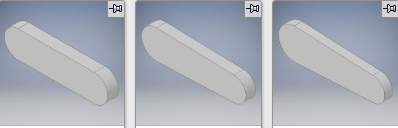
\includegraphics[scale=1]{Imagenes/GL.png}\\1.2 Antebeasos de grados de libertad
\end{center}
Utilizando el programa Autodesk Inventor y las referencias anteriormente mencionadas puede quedar de la siguiente manera:\\
\begin{center}
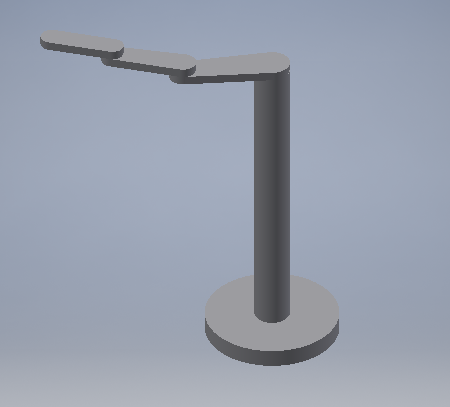
\includegraphics[scale=1]{Imagenes/AR.png}\\ 1.3 diseño brazo SCARA
\end{center}
Todo esto se sustentara sobre una base circulas de acero con espesor de 5mm y un peso aproximado de 12Kg para que el robot pueda mantenerce estale y cargar el peso establecido por el docente.\\
El resultado final que tuvimos al hacer una "Simulación" es positiva ya que mantiene un equilibrio estable y los servomotores poseen una capacidad de poder mover los grados de libertad de los antebrazos de este robot.\\
\\
\textbf{Conclusiones}\\
•Un robot SCARA siempre sera un reto para un estudiante sin importar que grado tenga, ya que la mayoria de este tipo de robot esta con un 75 de matem´aticas exactas para su buen funcionamiento, y tomando en cuenta los materiales a utilizar no solo sera un reto si no un aprendizaje del cual dejara muchos conocimientos que no pudieramos haber imaginado.\\
\\
•En terminos sencillos, cuando se trata de hacer que algo que puedes crear, tenga una utilidad, resulta bastante sencillo el poder crear una situación compleja donde la solución sea la creación en cuestión, en pocas palabras, el robot SCARA.\\
\\
•Los robots scara tienen una gran utilidad en la indusrtria por su rapides y su precicion, ahora  tenemos el reto de realizar un casi desde cero pero ahorita nomas hicimos el diseño en el que nos vamos a vasar, todavia nos falatan muchos pasos pero primero hay que comenzar por algo.\\
\\
•Para mi esto es solo una pequeña parte unicamente del diseño del robot, pero aun tenemos un camino largo por recorrer para lograr el objetivo y con ello las metas y objetimos que tenemos en mente.\\
\cite{vivas2006control}
\bibliographystyle{apalike} 
\bibliography{BIB}
\end{document}